\documentclass[tikz,border=2pt]{standalone}
\usepackage{amsmath}
\definecolor{pOrange}{RGB}{211,153,80}

% The marked Motzkin path U H D \bar{H} of length 4 (top) and the Dyck path
% U UU DU DD UD D of semilength 5 obtained by doubling it (bottom).  The steps
% of the Motzkin path sit above the step pairs they produce; up-steps in even
% positions are orange and each up-step is labelled by the height a_i before it.

\begin{document}
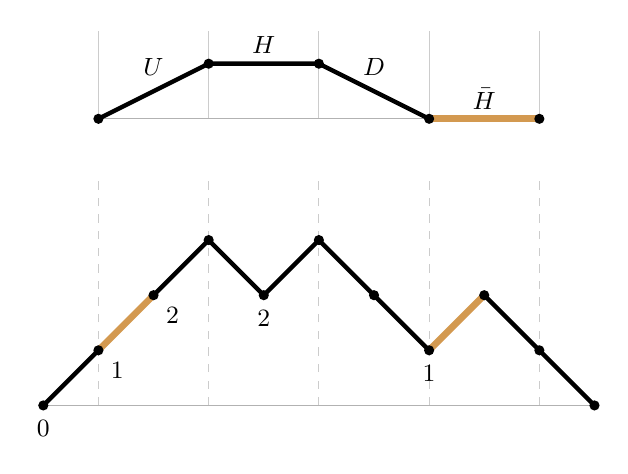
\begin{tikzpicture}[scale=0.7,
  dot/.style={circle,fill=black,inner sep=1.3pt},
  lab/.style={font=\small}]

  % ---------- Motzkin path, above ----------
  \begin{scope}[yshift=5.2cm]
    \foreach \x in {1,3,...,9} \draw[gray!40] (\x,0) -- (\x,1.6);
    \draw[gray!60] (1,0) -- (9,0);
    \draw[line width=1.6pt] (1,0) -- (3,1) -- (5,1) -- (7,0);
    \draw[line width=2.4pt,pOrange] (7,0) -- (9,0);
    \foreach \p in {(1,0),(3,1),(5,1),(7,0),(9,0)} \node[dot] at \p {};
    \node[lab,above] at (2,0.6) {$U$};
    \node[lab,above] at (4,1) {$H$};
    \node[lab,above] at (6,0.6) {$D$};
    \node[lab,above] at (8,0) {$\bar{H}$};
  \end{scope}

  % ---------- Dyck path, below ----------
  \foreach \x in {1,3,...,9} \draw[gray!40,dashed] (\x,0) -- (\x,4.2);
  \draw[gray!60] (0,0) -- (10,0);
  % up-steps at positions 1,2,3,5,8; positions 2 and 8 are even
  \draw[line width=1.6pt] (0,0) -- (1,1);
  \draw[line width=2.4pt,pOrange] (1,1) -- (2,2);
  \draw[line width=1.6pt] (2,2) -- (3,3) -- (4,2) -- (5,3) -- (6,2) -- (7,1);
  \draw[line width=2.4pt,pOrange] (7,1) -- (8,2);
  \draw[line width=1.6pt] (8,2) -- (9,1) -- (10,0);
  \foreach \p in {(0,0),(1,1),(2,2),(3,3),(4,2),(5,3),(6,2),(7,1),(8,2),(9,1),(10,0)}
    \node[dot] at \p {};
  % heights a_0,...,a_4 before the up-steps
  \node[lab,below=2pt] at (0,0) {$0$};
  \node[lab,below right=1pt] at (1,1) {$1$};
  \node[lab,below right=1pt] at (2,2) {$2$};
  \node[lab,below=2pt] at (4,2) {$2$};
  \node[lab,below=2pt] at (7,1) {$1$};
\end{tikzpicture}
\end{document}
